\documentclass[a4paper]{article}
\usepackage[]{graphicx}\usepackage[]{color}
% maxwidth is the original width if it is less than linewidth
% otherwise use linewidth (to make sure the graphics do not exceed the margin)
\makeatletter
\def\maxwidth{ %
  \ifdim\Gin@nat@width>\linewidth
    \linewidth
  \else
    \Gin@nat@width
  \fi
}
\makeatother

\definecolor{fgcolor}{rgb}{0.345, 0.345, 0.345}
\newcommand{\hlnum}[1]{\textcolor[rgb]{0.686,0.059,0.569}{#1}}%
\newcommand{\hlstr}[1]{\textcolor[rgb]{0.192,0.494,0.8}{#1}}%
\newcommand{\hlcom}[1]{\textcolor[rgb]{0.678,0.584,0.686}{\textit{#1}}}%
\newcommand{\hlopt}[1]{\textcolor[rgb]{0,0,0}{#1}}%
\newcommand{\hlstd}[1]{\textcolor[rgb]{0.345,0.345,0.345}{#1}}%
\newcommand{\hlkwa}[1]{\textcolor[rgb]{0.161,0.373,0.58}{\textbf{#1}}}%
\newcommand{\hlkwb}[1]{\textcolor[rgb]{0.69,0.353,0.396}{#1}}%
\newcommand{\hlkwc}[1]{\textcolor[rgb]{0.333,0.667,0.333}{#1}}%
\newcommand{\hlkwd}[1]{\textcolor[rgb]{0.737,0.353,0.396}{\textbf{#1}}}%
\let\hlipl\hlkwb

\usepackage{framed}
\makeatletter
\newenvironment{kframe}{%
 \def\at@end@of@kframe{}%
 \ifinner\ifhmode%
  \def\at@end@of@kframe{\end{minipage}}%
  \begin{minipage}{\columnwidth}%
 \fi\fi%
 \def\FrameCommand##1{\hskip\@totalleftmargin \hskip-\fboxsep
 \colorbox{shadecolor}{##1}\hskip-\fboxsep
     % There is no \\@totalrightmargin, so:
     \hskip-\linewidth \hskip-\@totalleftmargin \hskip\columnwidth}%
 \MakeFramed {\advance\hsize-\width
   \@totalleftmargin\z@ \linewidth\hsize
   \@setminipage}}%
 {\par\unskip\endMakeFramed%
 \at@end@of@kframe}
\makeatother

\definecolor{shadecolor}{rgb}{.97, .97, .97}
\definecolor{messagecolor}{rgb}{0, 0, 0}
\definecolor{warningcolor}{rgb}{1, 0, 1}
\definecolor{errorcolor}{rgb}{1, 0, 0}
\newenvironment{knitrout}{}{} % an empty environment to be redefined in TeX

\usepackage{alltt}
\newcommand{\SweaveOpts}[1]{}  % do not interfere with LaTeX
\newcommand{\SweaveInput}[1]{} % because they are not real TeX commands
\newcommand{\Sexpr}[1]{}       % will only be parsed by R




\usepackage[utf8]{inputenc}
%\usepackage[ngerman]{babel}
\usepackage{a4wide,paralist}
\usepackage{amsmath, amssymb, xfrac, amsthm}
\usepackage{dsfont}
\usepackage[usenames,dvipsnames]{xcolor}
\usepackage{amsfonts}
\usepackage{graphicx}
\usepackage{caption}
\usepackage{subcaption}
\usepackage{framed}
\usepackage{multirow}
\usepackage{bytefield}
\usepackage{csquotes}
\usepackage[breakable, theorems, skins]{tcolorbox}
\usepackage{hyperref}
\usepackage{cancel}
\usepackage{bm}


\input{../../style/common}

\tcbset{enhanced}

\DeclareRobustCommand{\mybox}[2][gray!20]{%
	\iffalse
	\begin{tcolorbox}[   %% Adjust the following parameters at will.
		breakable,
		left=0pt,
		right=0pt,
		top=0pt,
		bottom=0pt,
		colback=#1,
		colframe=#1,
		width=\dimexpr\linewidth\relax,
		enlarge left by=0mm,
		boxsep=5pt,
		arc=0pt,outer arc=0pt,
		]
		#2
	\end{tcolorbox}
	\fi
}

\DeclareRobustCommand{\myboxshow}[2][gray!20]{%
%	\iffalse
	\begin{tcolorbox}[   %% Adjust the following parameters at will.
		breakable,
		left=0pt,
		right=0pt,
		top=0pt,
		bottom=0pt,
		colback=#1,
		colframe=#1,
		width=\dimexpr\linewidth\relax,
		enlarge left by=0mm,
		boxsep=5pt,
		arc=0pt,outer arc=0pt,
		]
		#2
	\end{tcolorbox}
%	\fi
}


%exercise numbering
\renewcommand{\theenumi}{(\alph{enumi})}
\renewcommand{\theenumii}{\roman{enumii}}
\renewcommand\labelenumi{\theenumi}


\font \sfbold=cmssbx10

\setlength{\oddsidemargin}{0cm} \setlength{\textwidth}{16cm}


\sloppy
\parindent0em
\parskip0.5em
\topmargin-2.3 cm
\textheight25cm
\textwidth17.5cm
\oddsidemargin-0.8cm
\pagestyle{empty}

\newcommand{\kopf}[1] {
\hrule
\vspace{.15cm}
\begin{minipage}{\textwidth}
%akwardly i had to put \" here to make it compile correctly
	{\sf\bf Introduction to Machine Learning \hfill Exercise sheet #1\\
	 \url{https://introduction-to-machine-learning.netlify.app/} \hfill WiSe 2020/2021}
\end{minipage}
\vspace{.05cm}
\hrule
\vspace{1cm}}

\newenvironment{allgemein}
	{\noindent}{\vspace{1cm}}

\newcounter{aufg}
\newenvironment{aufgabe}
	{\refstepcounter{aufg}\textbf{Exercise \arabic{aufg}:}\\ \noindent}
	{\vspace{0.5cm}}

\newcounter{loes}
\newenvironment{loesung}
	{\refstepcounter{loes}\textbf{Solution \arabic{loes}:}\\\noindent}
	{\bigskip}
	
\newenvironment{bonusaufgabe}
	{\refstepcounter{aufg}\textbf{Exercise \arabic{aufg}*\footnote{This
	is a bonus exercise.}:}\\ \noindent}
	{\vspace{0.5cm}}

\newenvironment{bonusloesung}
	{\refstepcounter{loes}\textbf{Solution \arabic{loes}*:}\\\noindent}
	{\bigskip}



\begin{document}
% !Rnw weave = knitr



\input{../../latex-math/basic-math.tex}
\input{../../latex-math/basic-ml.tex}

\kopf{2}
\aufgabe{

%x <- c(4,7,9,4,6,7,9,7,8)
%y <- c(6,3,8,9,5,8,7,6,5)
%z <- as.factor(c(1,1,1,0,0,0,0,2,1))

Let the 2D feature vectors in the following figure be with two different numeric target values (2 and 4). Predict the point (7,6) - represented by the grey point in the picture - with the k-nearest neighbor method. Distance function should be the $L_1$ norm (Manhattan distance):

$$d_\text{manhattan}(x, \tilde{x}) = \sum_{j=1}^p |x_j - \tilde{x}_j|$$

State as the prediction the unweighted and the weighted (according to the Manhattan distance) mean of the values of the k-nearest neighbors.

\begin{itemize}
  \item[a)] $k = 3$
  \item[b)] $k = 5$
  \item[c)] $k = 7$
\end{itemize}

%d3 = c(5,7,9,7)
%v3 = c(6,8,6,4)

%d5 = c(4,7,10,7)
%v5 = c(6,9,6,3)

%d7 = c(3,7,10,10,7)
%v7 = c(6,10,7,5,2)



\begin{knitrout}
\definecolor{shadecolor}{rgb}{0.969, 0.969, 0.969}\color{fgcolor}

{\centering 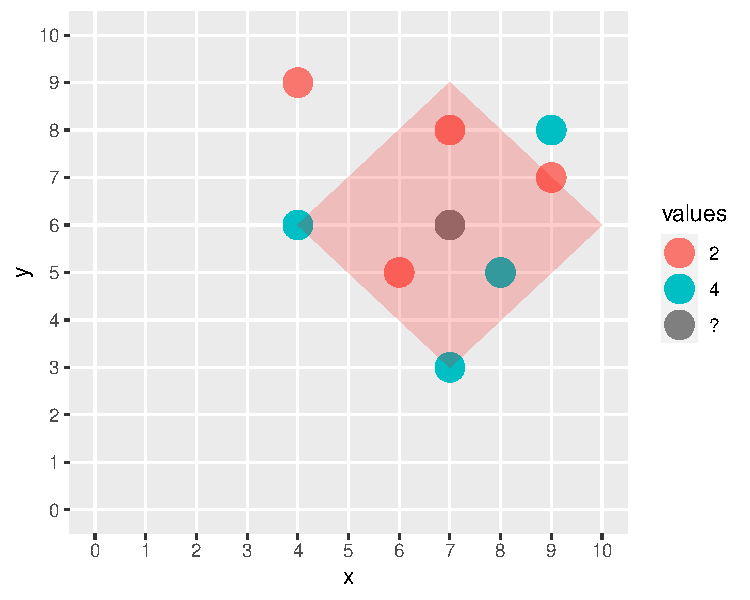
\includegraphics[width=\maxwidth]{figure/unnamed-chunk-4-1} 

}


\end{knitrout}
}

\dlz

\pagebreak 

\aufgabe{

How in mlr3 a learner can be constructed and what it represents can be found 
at \url{https://mlr3book.mlr-org.com/learners.html}.
\begin{enumerate}
\item[a)] How does a learner in mlr3 compare to what you've learned in the videos?
\item[b)] Pick an mlr3 learner of your choice. What are the different settings for this learner? \\ 
(Hint: Use \texttt{mlr\_learners\$keys()} to see all available learners)
\end{enumerate}
}

\dlz

\aufgabe{

We want to predict the age of an abalone using its longest shell measurement and its weight.

See: \url{http://archive.ics.uci.edu/ml/datasets/Abalone} for more details.

\begin{itemize}
  \item[a)] Plot \texttt{LongestShell}, \texttt{WholeWeight} on the $x$- and $y$-axis and color points with \texttt{Rings}
\end{itemize}

  Using the mlr3-package:

\begin{itemize}
  \item[b)] Fit a linear model
  \item[c)] Fit a k-nearest-neighbors model
  \item[d)] Compare the fitted and observed targets for lm and knn, respectively (Hint: Use \texttt{autoplot()})
  % \item[e)] Compare which model performs better.
\end{itemize}

Hint: See the official book manual of the mlr3 package for usage:
\begin{center}
\url{https://mlr3book.mlr-org.com/index.html}
\end{center}
}
\end{document}
